\documentclass{article}
\usepackage{graphicx}
\usepackage[margin=1.5cm]{geometry}
\usepackage{amsmath}

\begin{document}
\twocolumn

\title{Tuesday Reading Assessment: Unit 0, Review of 135A}
\author{Prof. Jordan C. Hanson}

\maketitle

\section{Memory Bank}

\begin{itemize}
\item $\vec{a} = a_x \hat{i} + a_y \hat{j}$ ... Component notation for 2D vector
\item $\vec{a} + \vec{b} = (a_x + b_x)\hat{i} + (a_y + b_y)\hat{j}$ ... Adding vectors
\item $\vec{a} - \vec{b} = (a_x - b_x)\hat{i} + (a_y - b_y)\hat{j}$ ... Subtracting vectors
\item $|\vec{a}| = \sqrt{a_x^2 + a_y^2}$ .. Magnitude of a 2D vector
\item $a_x = |\vec{a}|\cos\theta$ ... x-component of a 2D vector
\item $a_y = |\vec{a}|\sin\theta$ ... y-component of a 2D vector
\item \textbf{Couloumb's Law}: Let two charges with magnitudes $q_1$ and $q_2$ be separated by a displacement $\vec{r}$.  The force between them is 
\begin{equation}
\vec{F} = \frac{k q_1 q_2}{r^2}\hat{r}
\end{equation}
The vector $\hat{r}$ is a unit vector in the direction of $\vec{r}$, and $r$ is the magnitude.  The constant $k$ is $k=8.988 \times 10^9$ N m$^2$ C$^{-1}$.
\item $\vec{F} = q\vec{E}$ ... The electric field $\vec{E}$ causes the Coulomb force on a charge $q$.
\item \textbf{Couloumb Field}: Let a charge with magnitude $q$ be separated by a displacement $\vec{r}$ from a \textit{test charge}.  The E-field generated by $q$ is 
\begin{equation}
\vec{E} = \frac{k q}{r^2}\hat{r}
\end{equation}
The vector $\hat{r}$ is a unit vector in the direction of $\vec{r}$, and $r$ is the magnitude.  The constant $k$ is $k=8.988 \times 10^9$ N m$^2$ C$^{-1}$.
\end{itemize}

\section{Warm-Up Exercises}

\begin{enumerate}
\item Perform the following unit conversions:
\begin{itemize}
\item Convert 320 gm to kg:
\item Convert $2.4 \times 10^{5}$ cm s$^{-1}$ to km hr$^{-1}$:
\item Convert the density of ice, $0.9167$ gm cm$^{-3}$, to kg m$^{-3}$. \\ \vspace{0.5cm}
\end{itemize}
\item Let $\vec{x} = 0.5 \hat{i} - 0.5\hat{j}$, and $\vec{y} = -0.5\hat{i} + 0.5\hat{j}$. (a) Calculate $\vec{x} + \vec{y}$.  (b) Calculate $\vec{x} - \vec{y}$. (c) What is the magnitude of $\vec{a}$? (d) What is the magnitude of $\vec{b}$? \\ \vspace{2cm}
\item Let $\vec{F}$ be a 10 N force that makes a 60 degree angle with the x-axis. (a) What is the x-component of this force? (b) What is the y-component? (c) Suppose this force displaces a system 3 m along the x-axis.  What is the work done?  \textit{Recall that $W = \vec{F} \cdot \Delta \vec{x}$.} \\ \vspace{3cm}
\item Suppose a charge $q_1 = -1$ nC is located 1 cm away from a charge $q_2 = +1$ nC.  What is the magnitude and direction of the force between the charges?  To interpret the direction, consider Fig. \ref{fig:1}. \\ \vspace{3cm}
\item Suppose four equal charges $q$ form a square with side length $a$.  What is the magnitude of the electric field at the center of the square?
\end{enumerate}

\begin{figure}
\centering
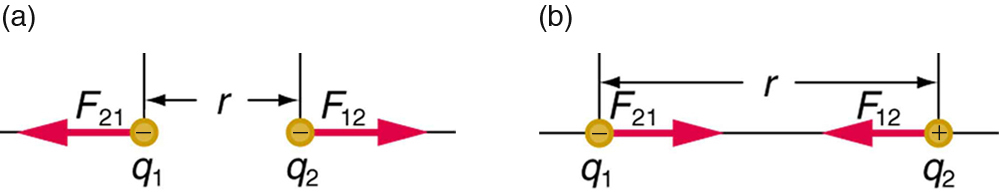
\includegraphics[width=0.5\textwidth]{figures/force.jpeg}
\caption{\label{fig:1} Coulomb forces between charges.}
\end{figure}

\end{document}
